\documentclass[aspectratio=169,11pt]{beamer}

% =============================================================================
% 1. PRESENTATION METADATA CONFIGURATION (EDIT FOR EACH REVIEW)
% =============================================================================
\newcommand{\reviewBanner}{EVALUATION II}                          % e.g., EVALUATION I, II, III, FINAL DEFENSE
\newcommand{\presentationTitle}{UNLIMITED SAMPLING-BASED HIGH-DYNAMIC-RANGE\\SPEECH ACQUISITION AND RECONSTRUCTION UNDER\\PRACTICAL ADC CONDITIONS}
\newcommand{\presentationSubtitle}{23ECE498 \& 23EAC498 --- PROJECT PHASE I}
\newcommand{\academicYear}{AY 2026--2027}

% Team Member Credentials
\newcommand{\memberOneRoll}{BL.EN.U4ECE23205}
\newcommand{\memberOneName}{Chandan Sai Pavan Padala}
\newcommand{\memberTwoRoll}{BL.EN.U4ECE23226}
\newcommand{\memberTwoName}{M Madhumitha}
\newcommand{\memberThreeRoll}{BL.EN.U4ECE23227}
\newcommand{\memberThreeName}{M V Sri Harsha}

% Faculty & Evaluation Panel
\newcommand{\guideName}{Dr. S. Lalitha}
\newcommand{\evaluatorOne}{Dr. Susmitha Vekkot}
\newcommand{\evaluatorTwo}{Dr. Vivek Venugopal}

% Footer Branding & University Credentials
\newcommand{\footerTeamName}{Team DHV\={A}N\={I}}                  % Displayed bottom-left
\newcommand{\departmentName}{Department of Electronics and Communication Engineering}
\newcommand{\campusName}{Amrita School of Engineering, Bengaluru \quad$\bullet$\quad Amrita Vishwa Vidyapeetham}

% Logo Asset Selection (color, dark, or white)
\newcommand{\logoAsset}{Amrita-vishwa-vidyapeetham-dark-logo.png}

% Optional Background: Comment out to use clean white academic background
\def\useGradientBackground{1}

% =============================================================================
% 2. THEME & PACKAGE INCLUSION
% =============================================================================
\usepackage{beamer_amrita_theme}
\usepackage[none]{hyphenat}
\hyphenpenalty=10000
\exhyphenpenalty=10000
\binoppenalty=10000
\relpenalty=10000
\tolerance=10000
\emergencystretch=3em
\righthyphenmin=62
\lefthyphenmin=62

% Background Canvas (Seamless switch between Gradient or Clean Canvas)
\setbeamertemplate{background}{%
  \ifdefined\useGradientBackground
    \begin{tikzpicture}[remember picture, overlay]
      \fill[canvasBg] (current page.south west) rectangle (current page.north east);
      \node[anchor=center, inner sep=0pt] at (current page.center) {%
        
\includegraphics[width=\paperwidth, height=\paperheight, keepaspectratio=false]{background-gradient.png}%
      };
    \end{tikzpicture}%
  \fi
}

% =============================================================================
% DOCUMENT CONTENT
% =============================================================================
\begin{document}

% -----------------------------------------------------------------------------
% FRAME 1: MASTER TITLE SLIDE
% -----------------------------------------------------------------------------
\begin{frame}[t]
  \vspace*{-0.35cm}
  \noindent
  \hfill
  \begin{minipage}[c]{0.5\textwidth}
    \raggedleft
    \includegraphics[height=0.80cm, keepaspectratio]{\logoAsset}%
    \hspace*{-0.80cm}%
  \end{minipage}%

  \vspace{0.08cm}
  \begin{glasscard}[opacityback=0.18, arc=3.5mm, top=6pt, bottom=6pt, left=8pt, right=8pt]
    \begin{center}
      \tikz\node[draw=accentDark, line width=1.2pt, rounded corners=4pt, fill=white, fill opacity=0.65, text opacity=1, inner xsep=14pt, inner ysep=4pt]{%
        {\fontsize{12.5pt}{14.5pt}\selectfont\bfseries\color{accentDark} \reviewBanner}%
      };
      \vspace{0.14cm}

      {\fontsize{12pt}{15.5pt}\selectfont\bfseries\color{textPrimary} \presentationTitle}
      \vspace{0.14cm}

      \noindent
      {\color{accentDark}\rule[3pt]{0.12\linewidth}{1.2pt}} \quad
      {\fontsize{10pt}{12pt}\selectfont\bfseries\color{textPrimary} \presentationSubtitle} \quad
      {\color{accentDark}\rule[3pt]{0.12\linewidth}{1.2pt}}
    \end{center}
  \end{glasscard}

  \vspace{0.08cm}
  \begin{columns}[T]
    \begin{column}{0.49\textwidth}
      \begin{glasscard}[top=4pt, bottom=4pt, left=6pt, right=6pt]
        {\color{accentDark}\rule[-1pt]{2.5pt}{9pt}}\hspace{5pt}%
        {\fontsize{9pt}{11pt}\selectfont\bfseries\color{textPrimary} TEAM MEMBERS:}\\[3pt]
        {\fontsize{8.5pt}{11pt}\selectfont\color{textPrimary}
        \memberOneRoll\ --- \memberOneName\\
        \memberTwoRoll\ --- \memberTwoName\\
        \memberThreeRoll\ --- \memberThreeName}
      \end{glasscard}
    \end{column}
    \begin{column}{0.49\textwidth}
      \begin{glasscard}[top=4pt, bottom=4pt, left=6pt, right=6pt]
        {\color{accentDark}\rule[-1pt]{2.5pt}{9pt}}\hspace{5pt}%
        {\fontsize{9pt}{11pt}\selectfont\bfseries\color{textPrimary} PROJECT SUPERVISION:}\\[3pt]
        {\fontsize{8.5pt}{11pt}\selectfont\color{textPrimary}
        \textbf{\color{textPrimary}Name of the Guide:}\hspace{1.8em} \color{textPrimary}\guideName\\[2pt]
        \textbf{\color{textPrimary}Name of the Evaluators:}\ \color{textPrimary}\evaluatorOne\\
        \phantom{\textbf{Name of the Evaluators:}}\ \color{textPrimary}\evaluatorTwo}
      \end{glasscard}
    \end{column}
  \end{columns}
\end{frame}

% -----------------------------------------------------------------------------
% FRAME 2: AGENDA / TABLE OF CONTENTS (BENTO GRID STYLE)
% -----------------------------------------------------------------------------
\begin{frame}[t]
  \vspace*{-0.35cm}
  \noindent
  \hfill
  \begin{minipage}[c]{0.5\textwidth}
    \raggedleft
    \includegraphics[height=0.80cm, keepaspectratio]{\logoAsset}%
    \hspace*{-0.80cm}%
  \end{minipage}%

  \vspace{0.05cm}
  \begin{center}
    {\color{accentDark}\rule[3.5pt]{0.14\linewidth}{1.2pt}} \hspace{0.5em}
    {\fontsize{15pt}{17pt}\selectfont\bfseries\color{textPrimary} TABLE OF CONTENTS} \hspace{0.5em}
    {\color{accentDark}\rule[3.5pt]{0.14\linewidth}{1.2pt}}
  \end{center}
  \vspace{0.08cm}

  \begin{columns}[onlytextwidth]
    \begin{column}{0.485\textwidth}
      \begin{glasscard}[boxsep=1.2pt, top=1.8pt, bottom=1.8pt, left=6pt, right=6pt]
        \tikz\node[rounded corners=2pt, draw=black!70, line width=0.5pt, fill=white, fill opacity=0.75, text opacity=1, text=black, font=\bfseries\scriptsize, inner xsep=3.5pt, inner ysep=1pt]{01.};
        \hspace{0.4em}{\fontsize{8.5pt}{10.5pt}\selectfont\textbf{\color{textPrimary}Introduction \& Acoustic Motivation}}
      \end{glasscard}
      \vspace{2.5pt}

      \begin{glasscard}[boxsep=1.2pt, top=1.8pt, bottom=1.8pt, left=6pt, right=6pt]
        \tikz\node[rounded corners=2pt, draw=black!70, line width=0.5pt, fill=white, fill opacity=0.75, text opacity=1, text=black, font=\bfseries\scriptsize, inner xsep=3.5pt, inner ysep=1pt]{02.};
        \hspace{0.4em}{\fontsize{8.5pt}{10.5pt}\selectfont\textbf{\color{textPrimary}Unlimited Sampling Theoretical Bounds}}
      \end{glasscard}
      \vspace{2.5pt}

      \begin{glasscard}[boxsep=1.2pt, top=1.8pt, bottom=1.8pt, left=6pt, right=6pt]
        \tikz\node[rounded corners=2pt, draw=black!70, line width=0.5pt, fill=white, fill opacity=0.75, text opacity=1, text=black, font=\bfseries\scriptsize, inner xsep=3.5pt, inner ysep=1pt]{03.};
        \hspace{0.4em}{\fontsize{8.5pt}{10.5pt}\selectfont\textbf{\color{textPrimary}Project Objectives \& Phased Deliverables}}
      \end{glasscard}
      \vspace{2.5pt}

      \begin{glasscard}[boxsep=1.2pt, top=1.8pt, bottom=1.8pt, left=6pt, right=6pt]
        \tikz\node[rounded corners=2pt, draw=black!70, line width=0.5pt, fill=white, fill opacity=0.75, text opacity=1, text=black, font=\bfseries\scriptsize, inner xsep=3.5pt, inner ysep=1pt]{04.};
        \hspace{0.4em}{\fontsize{8.5pt}{10.5pt}\selectfont\textbf{\color{textPrimary}Literature Review \& Baseline Benchmarks}}
      \end{glasscard}
      \vspace{2.5pt}

      \begin{glasscard}[boxsep=1.2pt, top=1.8pt, bottom=1.8pt, left=6pt, right=6pt]
        \tikz\node[rounded corners=2pt, draw=black!70, line width=0.5pt, fill=white, fill opacity=0.75, text opacity=1, text=black, font=\bfseries\scriptsize, inner xsep=3.5pt, inner ysep=1pt]{05.};
        \hspace{0.4em}{\fontsize{8.5pt}{10.5pt}\selectfont\textbf{\color{textPrimary}End-to-End System Architecture}}
      \end{glasscard}
    \end{column}

    \begin{column}{0.485\textwidth}
      \begin{glasscard}[boxsep=1.2pt, top=1.8pt, bottom=1.8pt, left=6pt, right=6pt]
        \tikz\node[rounded corners=2pt, draw=black!70, line width=0.5pt, fill=white, fill opacity=0.75, text opacity=1, text=black, font=\bfseries\scriptsize, inner xsep=3.5pt, inner ysep=1pt]{06.};
        \hspace{0.4em}{\fontsize{8.5pt}{10.5pt}\selectfont\textbf{\color{textPrimary}Modular DSP Simulation Core (\texttt{src/})}}
      \end{glasscard}
      \vspace{2.5pt}

      \begin{glasscard}[boxsep=1.2pt, top=1.8pt, bottom=1.8pt, left=6pt, right=6pt]
        \tikz\node[rounded corners=2pt, draw=black!70, line width=0.5pt, fill=white, fill opacity=0.75, text opacity=1, text=black, font=\bfseries\scriptsize, inner xsep=3.5pt, inner ysep=1pt]{07.};
        \hspace{0.4em}{\fontsize{8.5pt}{10.5pt}\selectfont\textbf{\color{textPrimary}Synthetic Multi-Tone Inversion Proof}}
      \end{glasscard}
      \vspace{2.5pt}

      \begin{glasscard}[boxsep=1.2pt, top=1.8pt, bottom=1.8pt, left=6pt, right=6pt]
        \tikz\node[rounded corners=2pt, draw=black!70, line width=0.5pt, fill=white, fill opacity=0.75, text opacity=1, text=black, font=\bfseries\scriptsize, inner xsep=3.5pt, inner ysep=1pt]{08.};
        \hspace{0.4em}{\fontsize{8.5pt}{10.5pt}\selectfont\textbf{\color{textPrimary}Hardware Robustness \& Stress Ablations}}
      \end{glasscard}
      \vspace{2.5pt}

      \begin{glasscard}[boxsep=1.2pt, top=1.8pt, bottom=1.8pt, left=6pt, right=6pt]
        \tikz\node[rounded corners=2pt, draw=black!70, line width=0.5pt, fill=white, fill opacity=0.75, text opacity=1, text=black, font=\bfseries\scriptsize, inner xsep=3.5pt, inner ysep=1pt]{09.};
        \hspace{0.4em}{\fontsize{8.5pt}{10.5pt}\selectfont\textbf{\color{textPrimary}Speech Ingestion \& Emotional Corpus}}
      \end{glasscard}
      \vspace{2.5pt}

      \begin{glasscard}[boxsep=1.2pt, top=1.8pt, bottom=1.8pt, left=6pt, right=6pt]
        \tikz\node[rounded corners=2pt, draw=black!70, line width=0.5pt, fill=white, fill opacity=0.75, text opacity=1, text=black, font=\bfseries\scriptsize, inner xsep=3.5pt, inner ysep=1pt]{10.};
        \hspace{0.4em}{\fontsize{8.5pt}{10.5pt}\selectfont\textbf{\color{textPrimary}Phase 2 Milestones \& Roadmap}}
      \end{glasscard}
    \end{column}
  \end{columns}
\end{frame}

% -----------------------------------------------------------------------------
% FRAME 3: STANDARD 2-COLUMN SLIDE (PROBLEM & CONCEPT)
% -----------------------------------------------------------------------------
\begin{frame}[t]
  \slideheader{THE ACOUSTIC DILEMMA: CLIPPING}
  \vspace*{-0.10cm}

  \begin{columns}[T, onlytextwidth]
    \begin{column}{0.485\textwidth}
      \begin{glassbox}[top=4pt, bottom=4pt, left=6pt, right=6pt, title=\textbf{Acoustic Clipping Bottleneck}]{}
        \fontsize{8.2pt}{10.5pt}\selectfont
        \begin{itemize}\setlength{\itemsep}{2pt}
          \item \textbf{Finite Rail Saturation:} Traditional ADCs irreversibly flatten amplitudes when $|x(t)| > \lambda$, permanently destroying spectral crests.
          \item \textbf{Harmonic Splatter:} Sharp rail transitions generate spurious high-frequency harmonics, distorting formant striations.
          \item \textbf{Downstream Failure:} Saturated signals degrade intelligibility, causing catastrophic word error rate (WER) penalties in ASR.
        \end{itemize}
      \end{glassbox}
    \end{column}

    \begin{column}{0.485\textwidth}
      \begin{imagebox}{4.65cm}
        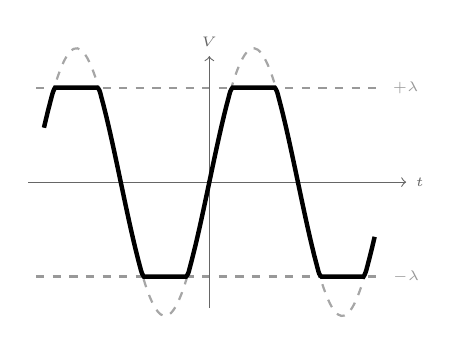
\begin{tikzpicture}
          \draw[dashed, black!40, thick] (-2.2, 1.2) -- (2.2, 1.2) node[right, font=\tiny] {$+\lambda$};
          \draw[dashed, black!40, thick] (-2.2, -1.2) -- (2.2, -1.2) node[right, font=\tiny] {$-\lambda$};
          \draw[->, black!60] (-2.3, 0) -- (2.5, 0) node[right, font=\tiny] {$t$};
          \draw[->, black!60] (0, -1.6) -- (0, 1.6) node[above, font=\tiny] {$V$};
          \draw[domain=-2.1:2.1, samples=100, smooth, black!35, thick, dashed] plot (\x, {1.7*sin(\x * 160)});
          \draw[domain=-2.1:2.1, samples=150, smooth, black, ultra thick] plot (\x, {max(-1.2, min(1.2, 1.7*sin(\x * 160)))});
        \end{tikzpicture}
      \end{imagebox}
      \vspace{2pt}
      {\centering\fontsize{7.5pt}{9.5pt}\selectfont\color{black!70}\textit{Figure 1. Hard clipping distortion and dynamic range saturation.}\par}
    \end{column}
  \end{columns}
\end{frame}

% -----------------------------------------------------------------------------
% FRAME 4: PROCESS / OBJECTIVES SLIDE (NUMBERED PROCESS PILLS)
% -----------------------------------------------------------------------------
\begin{frame}[t]
  \slideheader{OBJECTIVES \& PHASED DELIVERABLES}
  \vspace*{-0.05cm}

  \processcard{1}{Theoretical Bounds \& Contractive Sampling}{%
    Mathematically formulate the Unlimited Sampling Framework (USF), deriving exact contractive difference conditions ($\|\Delta^N x\|_\infty < \lambda$) based on Bernstein's inequality and resolving integer integration constants $\kappa_n \in 2\lambda\mathbb{Z}$.}
  \vspace{0.08cm}

  \processcard{2}{DSP Simulation Core \& Annihilating Filters}{%
    Develop modular, MathWorks-compliant MATLAB algorithms implementing centered modulo folding, higher-order difference unwrapping ($N = 1\dots 5$), and continuous-time Fourier-Prony spectral annihilating filters with Cadzow SVD rank reduction.}
  \vspace{0.08cm}

  \processcard{3}{Speech Dataset Benchmarking \& Intelligibility}{%
    Ingest real human speech under controlled folding factors ($\rho = 1\dots 6\times$); demonstrate 100\% vocal plosive recovery, spectrogram formant reconstruction, and perceptual metric retention (STOI, PESQ, LSD).}
\end{frame}

% -----------------------------------------------------------------------------
% FRAME 5: MATHEMATICAL FORMULATION SLIDE
% -----------------------------------------------------------------------------
\begin{frame}[t]
  \slideheader{THEORETICAL USF FORMULATION}
  \vspace*{-0.15cm}

  \begin{columns}[T, onlytextwidth]
    \begin{column}{0.485\textwidth}
      \begin{glassbox}[top=4pt, bottom=4pt, left=6pt, right=6pt, title=\textbf{Analytical Sampling Guarantee}]{}
        \fontsize{8.2pt}{10.5pt}\selectfont
        \textbf{Centered Modulo Folding Operator:}
        \begin{equation*}
          \mathcal{M}_\lambda(x) = \text{mod}(x + \lambda, 2\lambda) - \lambda \in [-\lambda, +\lambda]
        \end{equation*}
        \textbf{Bernstein Difference Condition:}
        \begin{equation*}
          \|\Delta^N x\|_\infty \le (T \pi e f_{\max})^N \|x\|_\infty < \lambda
        \end{equation*}
        \textbf{Critical Sampling Frequency Bound:}
        \begin{equation*}
          F_{\text{USF}} \ge 2\pi e f_{\max} \approx 17.08\,f_{\max}
        \end{equation*}
        Guarantees exact, unique integer phase unraveling.
      \end{glassbox}
    \end{column}

    \begin{column}{0.485\textwidth}
      \begin{glassbox}[top=4pt, bottom=4pt, left=6pt, right=6pt, title=\textbf{Variable \& Parameter Definitions}]{}
        \fontsize{7.5pt}{9.2pt}\selectfont
        \renewcommand{\arraystretch}{0.95}
        \begin{tabularx}{\linewidth}{>{\bfseries\color{textPrimary}}l >{\color{textPrimary}}X}
          \toprule
          Parameter & Physical Definition \\
          \midrule
          $\lambda$ & ADC dynamic rail voltage limit ($\pm 1.0\text{ V}$) \\
          $\rho = \|x\|_\infty / \lambda$ & Overload factor ($1\times \dots 6\times$ excursion) \\
          $N$ & Finite-difference contraction order ($N \ge 2$) \\
          $T = 1/F_s$ & Uniform sampling interval \\
          $f_{\max}$ & Maximum acoustic passband cutoff ($4\text{ kHz}$) \\
          $F_{\text{USF}}$ & USF critical contractive sampling rate \\
          \bottomrule
        \end{tabularx}
      \end{glassbox}
    \end{column}
  \end{columns}
\end{frame}

% -----------------------------------------------------------------------------
% FRAME 6: FULL-WIDTH GRAPHIC CONTAINER SLIDE
% -----------------------------------------------------------------------------
\begin{frame}[t]
  \slideheader{PARAMETRIC NOISE SWEEPS \& ROBUSTNESS}
  \vspace*{-0.10cm}

  \begin{center}
    \begin{imagebox}{4.75cm}
      \begin{tikzpicture}
        \draw[rounded corners=3pt, draw=black!25, dashed, line width=0.8pt] (-5.6, -1.8) rectangle (5.6, 1.8);
        \node[font=\small\bfseries\color{textPrimary}] at (0, 0.4) {[ Full-Width Visual / Experimental Results Placeholder ]};
        \node[font=\footnotesize\color{black!60}] at (0, -0.3) {Supports \texttt{\textbackslash includegraphics[width=0.90\textbackslash textwidth, height=4.5cm]\{...\}}};
      \end{tikzpicture}
    \end{imagebox}
    \vspace{3pt}
    {\fontsize{8.2pt}{10.2pt}\selectfont\color{black!75}\textit{Figure 2. Parametric analog input SNR sweeps validating stable reconstruction performance across diverse noise regimes.}}
  \end{center}
\end{frame}

% -----------------------------------------------------------------------------
% FRAME 7: COMPARATIVE BENCHMARK TABLE SLIDE
% -----------------------------------------------------------------------------
\begin{frame}[t]
  \slideheader{COMPARATIVE BENCHMARK: 5 METHODS}
  \vspace*{-0.10cm}

  \begin{glasscard}[top=3pt, bottom=3pt, left=4pt, right=4pt]
    \footnotesize
    \setlength{\tabcolsep}{3.5pt}
    \begin{tabularx}{\linewidth}{>{\bfseries\raggedright\arraybackslash\color{textPrimary}}p{2.85cm} >{\centering\arraybackslash\color{textPrimary}}X >{\centering\arraybackslash\color{textPrimary}}X >{\centering\arraybackslash\color{textPrimary}}c >{\centering\arraybackslash\color{textPrimary}}c >{\centering\arraybackslash\color{textPrimary}}X}
      \toprule
      \color{textPrimary} Method & \color{textPrimary} Peak Rule & \color{textPrimary} Phase Linearity & \color{textPrimary} SNR ($\rho{=}3.5$) & \color{textPrimary} STOI & \color{textPrimary} Complexity \\
      \midrule
      Standard Hard Clipping & Saturated ($\pm\lambda$) & Non-Linear Loss & $10.61\text{ dB}$ & $0.784$ & $\mathcal{O}(1)$ \\[2.5pt]
      Analog AGC & Delayed Pumping & Non-Linear Lag & $14.20\text{ dB}$ & $0.812$ & $\mathcal{O}(1)$ \\[2.5pt]
      $\mu$-Law Companding & Log Compression & Warped Dynamic & $18.50\text{ dB}$ & $0.865$ & $\mathcal{O}(N)$ \\[2.5pt]
      Cubic Spline (PCHIP) & Inpainted Spline & Smooth Error & $11.85\text{ dB}$ & $0.801$ & $\mathcal{O}(N^2)$ \\[2.5pt]
      \textbf{DHV\={A}N\={I} USF Hybrid} & \textbf{Lossless Fold} & \textbf{Exact Linear} & $\mathbf{48.26\text{ dB}}$ & $\mathbf{1.000}$ & $\mathcal{O}(N \log N)$ \\
      \bottomrule
    \end{tabularx}
  \end{glasscard}
  \vspace{3pt}
  \centering
  {\fontsize{8pt}{10pt}\selectfont\color{black!75}\textit{Table 1. Quantitative audio restoration performance across emotional speech categories under extreme $\rho = 3.50\times$ excursion.}}
\end{frame}

% -----------------------------------------------------------------------------
% FRAME 8: PROJECT ROADMAP & FUTURE MILESTONES
% -----------------------------------------------------------------------------
\begin{frame}[t]
  \slideheader{PROJECT ROADMAP \& FUTURE MILESTONES}
  \vspace*{-0.10cm}

  \begin{columns}[T, onlytextwidth]
    \begin{column}{0.485\textwidth}
      \begin{glassbox}[top=4pt, bottom=4pt, left=6pt, right=6pt, title=\textbf{Phase 1: Completed Deliverables}]{}
        \fontsize{8.2pt}{10.2pt}\selectfont
        \begin{itemize}\setlength{\itemsep}{2pt}
          \item \textbf{Mathematical Closure:} Proven finite-difference convergence under Bernstein contraction bounds.
          \item \textbf{DSP Engine:} 5 modular MATLAB algorithms verifying $160.8\text{ dB}$ SNR multi-tone recovery.
          \item \textbf{Ablation Suite:} Static DC bias invariance and coarse 8-bit quantization robustness.
          \item \textbf{Corpus Validation:} RAVDESS 6-emotion speech evaluation achieving $\text{STOI} = 1.000$.
        \end{itemize}
      \end{glassbox}
    \end{column}

    \begin{column}{0.485\textwidth}
      \begin{glassbox}[top=4pt, bottom=4pt, left=6pt, right=6pt, title=\textbf{Phase 2: Target Milestones}]{}
        \fontsize{8.2pt}{10.2pt}\selectfont
        \begin{itemize}\setlength{\itemsep}{2pt}
          \item \textbf{Hardware Prototype:} Fabricate and test 4-layer low-noise IBMADC PCB front-end.
          \item \textbf{Firmware Integration:} ESP32 dual-core 24-bit $96\text{ kHz}$ DMA ping-pong streaming buffer.
          \item \textbf{AI Gatekeeper:} 1D Dilated Residual ResNet ONNX model ($<250\text{k}$ params, $0.199\text{ ms}$ latency).
          \item \textbf{Downstream ASR:} Benchmarking WER retention on Whisper across high-noise folding regimes.
        \end{itemize}
      \end{glassbox}
    \end{column}
  \end{columns}
\end{frame}

% -----------------------------------------------------------------------------
% FRAME 9: FORMAL LITERATURE REFERENCES
% -----------------------------------------------------------------------------
\begin{frame}[t]
  \slideheader{REFERENCES}
  \vspace*{-0.20cm}

  \begin{glasscard}[top=3pt, bottom=3pt, left=7pt, right=7pt]
    {\color{accentLightBlue}\rule[-1pt]{2.5pt}{8pt}}\hspace{5pt}%
    {\fontsize{9pt}{11pt}\selectfont\bfseries\color{textPrimary} Foundational IEEE Literature:}\\[3pt]
    {\fontsize{7.6pt}{9.8pt}\selectfont\color{black!75}
    \textbf{[1]} A. Bhandari, F. Krahmer, and R. Raskar, ``On unlimited sampling and reconstruction,'' \textit{IEEE Transactions on Signal Processing}, vol. 69, pp. 3827--3839, 2021.\\[2pt]
    \textbf{[2]} A. Bhandari, F. Krahmer, and T. Poskitt, ``Unlimited sampling from theory to practice: Fourier-Prony recovery and hardware,'' \textit{IEEE Transactions on Signal Processing}, vol. 70, pp. 1131--1146, 2022.\\[2pt]
    \textbf{[3]} Y. Zhu, T. Poskitt, F. Krahmer, and A. Bhandari, ``The IBMADC: Architecture, circuit design, and recovery guarantees,'' \textit{IEEE Transactions on Circuits and Systems I: Regular Papers}, vol. 71, no. 5, pp. 2011--2024, 2024.\\[2pt]
    \textbf{[4]} C. H. Taal, R. C. Hendriks, R. Heusdens, and J. Jensen, ``An algorithm for predicting the intelligibility of speech of both normal and hearing-impaired listeners,'' \textit{IEEE Transactions on Audio, Speech, and Language Processing}, vol. 19, no. 7, pp. 2125--2136, 2011.\\[2pt]
    \textbf{[5]} S. R. Livingstone and F. A. Russo, ``The Ryerson Audio-Visual Database of Emotional Speech and Song (RAVDESS),'' \textit{PLoS ONE}, vol. 13, no. 5, p. e0196391, 2018.
    }
  \end{glasscard}
\end{frame}

% -----------------------------------------------------------------------------
% FRAME 10: CLOSING / DEFENSE Q&A
% -----------------------------------------------------------------------------
\begin{frame}[t]
  \vspace*{-0.35cm}
  \noindent
  \hfill
  \begin{minipage}[c]{0.5\textwidth}
    \raggedleft
    \includegraphics[height=0.80cm, keepaspectratio]{\logoAsset}%
    \hspace*{-0.80cm}%
  \end{minipage}%

  \vspace{0.70cm}
  \begin{center}
    \begin{glasscard}[opacityback=0.18, arc=4mm, top=16pt, bottom=16pt, left=18pt, right=18pt]
      \centering
      {\fontsize{28pt}{32pt}\selectfont\bfseries\color{textPrimary} THANK YOU}\\[8pt]
      {\color{accentDark}\rule[4pt]{0.25\linewidth}{1.5pt}}\\[6pt]
      {\fontsize{13pt}{16pt}\selectfont\color{textPrimary} Questions \& Technical Discussion}\\[14pt]
      {\fontsize{9pt}{12pt}\selectfont\color{black!75} \footerTeamName\ \quad|\quad \departmentName}\\
      {\fontsize{8.5pt}{11pt}\selectfont\color{black!60} \campusName}
    \end{glasscard}
  \end{center}
\end{frame}

\end{document}
